\chapter{Pattern Recognition with Neural Networks: Background and Implementation}

\epigraph{Nowadays, with technology coming into cricket, people start to analyse, and if you only have one or two tricks, people will start to line you up}{Jasprit Bumrah}

We begin this chapter by looking at the mathematical background of neural networks. More specifically, the construction of them using Linear Algebra, and then algorithms 
for training them. By ``training'', we mean updating the parameters associated with the network in order to improve their predictive accuracy. After this mathematical discussion, 
we look at using the \verb|neuralnet| package in R to implement a network, although the resulting network is dicussed in the next chapter. The chapter finishes with a discussion of 
time complexity of the algorithms used.

%Explain which langauges were chosen for each method and why

\section{A Brief Introduction to Neural Networks}
Neural networks (NNs) have been the subject to a lot of discussion and exploration in recent years. They are a machine learning method that is being applied to many problems
in all sorts of fields, such as finance \cite{nnstock} and medicine \cite{nncancer}.  
The network will be trained on run rate data, so for each game we have calculated the evolution of the run rate,
and then we have the overall score for that game in the final column of the matrix. An example of a network can be seen in Figure~\ref{nnexample1}. The first layer is the 
input layer, and the last layer gives the predictions. The middle layers are hidden and where the work of the network is done. \\

\begin{figure}
    \centering
    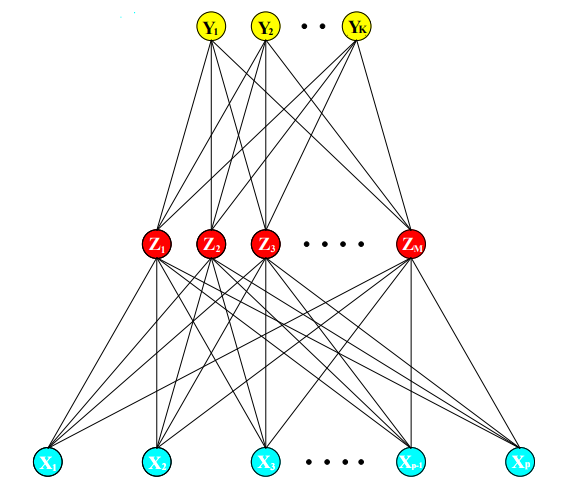
\includegraphics[scale=0.5]{figures/nn.png}
    \caption{Example of a single hidden layer neural network, as in \cite{sprbk}. Inputs are inputted through the bottom layer, the final activity value in the top
    layers are taken as the prediction.}
    \label{nnexample1}
\end{figure}

We see there are $p$ input nodes at the bottom, M nodes in the hidden layer, and K output layers. The lines between the layers are given a ``weight''
and a ``bias''. These properties will be discussed in more detail shortly. The number of hidden layers to be used will be the subject of experimentation. 
It's important to note how we will measure the success of the model. The main dataset, consisting of 1438 games of 50 overs is split into two subsets, one 
containing 70\% of the games, and one containing 30\%. We use the larger of the two to ``train'' the model, and the smaller one as a test set. Not doing this could 
lead to a phenomenom known as ``overfitting''; where the network learns how to predict patterns in the dataset it was trained on really well, but then isn't so good 
at predicting unseen values. We use correlation as the main metric of success in this model, which will be discussed later on.

As mentioned, NNs have been used extensively in finance- more specifically, in predicting future stock price behaviour. Naturally if one can predict how the value of a stock
will change over some time period, then one can protect themselfes from a bad investment, or profit heavily from a good one. We will use similar
methods here for building our neural network.  In \cite{nnstock}, the authors test two different Neural Networks, and find that using a ``Multi-Layer Feed Forward Nerual Network''
is the better choice for predicting how stock values will change. With these motivations in mind, we can begin to construct the networks.

\section{Building The Network}
Our input layer will have 50 nodes, one for the run rate at the end of each over. We will begin with 5 hidden layers, although this is subject to change. The output layer
will of course only have one node, the value of which will predict the score of the game. There will be three hidden layers, with 25, 10 and 3 nodes respectively. 
The ideas is that the prediction is refined over time down to a single value. In the future, more work is needed to experiment with different hidden layer topologies. 

We begin by looking at a single node. The proper name for each node is ``perceptron''. Each perceptron takes in the values of a vector, and an extra ``+1'' intercept term. The perceptron then outputs a value $h$ given by Equation~\ref{percepout}:

\begin{equation}
    \label{percepout}
    h_{W,b}(x) = f(\textbf{W}^Tx) = f(\sum_{i=1}^KW_ix_i+b).
\end{equation}

Here, $K \in \mathbb{N}$ is the number of elements in the vector, and $f:\mathbb{R} \rightarrow \mathbb{R}$ is called the activation function. There is a bit of choice in which activation function to use.
The two common choices are the Sigmoid function (Equation~\ref{sigmoid_func}) and the Hyperbolic Tangent Function:

\begin{align}
    \label{sigmoid_func}
    f(z) &= \frac{1}{1+exp(-z)} \\
    f(z) &= tanh(z)
\end{align}

The comparison of these two functions can be seen in Figure~\ref{actfig}.

\begin{figure}[h]
    \centering
    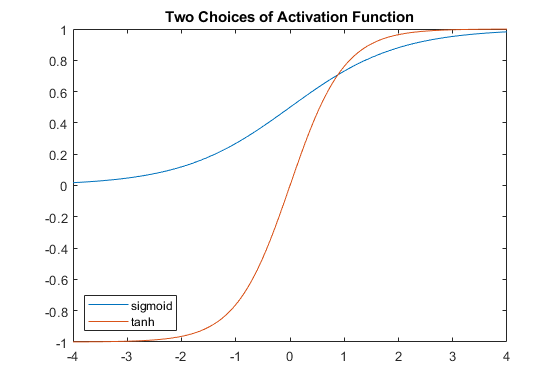
\includegraphics[scale=0.5]{figures/actfuncs.png}
    \caption{Graph showing the shape of different activation functions.}
    \label{actfig}
\end{figure}

We will be using Equation~\ref{sigmoid_func} as our activation function. There is some leniency over which activation function is used. The paper \cite{sibi} found that actually the more important aspect of 
the network is the choice of training algorithm, along with other parameters such as learning rate $\alpha$. For now, lets look at the network we're going to use. 

We begin with getting from the input layer, denoted $L_0$. Each node in $L_0$ takes a value $a^{(0)_i}$ for $i \in \{1,2,\ldots,50\}$. We use $\textbf{a}^{(0)}$ to denote the vector
containing these values. For every node in $L_0$, we have 25 connections coming away, one going to each of the nodes in $L_1$. 25 was an arbitrary choice for the size of $L_1$, and is
subject to change based on results from initial testing. So that means we have $50 \times 25 = 1250$ weights for just the first layer alone. Some linear algebra is to be done here to get 
values for the vector $\textbf{a}^{(1)}$. We use $w_{ij}$ to denote the weight from node j in one layer to node i in the prior layer. We can then construct a matrix containing the weights
between $L_0$ and $L_1$, which we denote $W^{(1)}$. This matrix is given by Equation~\ref{weights1}.

\begin{equation}
    W^{(1)} =
    \left[ {\begin{array}{cccc}
      w_{1,1} & w_{1,2} & \cdots & a_{1,50}\\
      w_{2,1} & w_{2,2} & \cdots & a_{2n}\\
      \vdots & \vdots & \ddots & \vdots\\
      w_{25,1} & a_{25,2} & \cdots & a_{25,50}\\
    \end{array} } \right]
    \label{weights1}
\end{equation}

Using Equation~\ref{weights1}, and combining with $a^{(0)}$, we can get the following:

\begin{align}
    A^{(1)} &= \left[ {\begin{array}{cccc}
        w_{1,1} & w_{1,2} & \cdots & a_{1,50}\\
        w_{2,1} & w_{2,2} & \cdots & a_{2n}\\
        \vdots & \vdots & \ddots & \vdots\\
        w_{25,1} & a_{25,2} & \cdots & a_{25,50}\\
      \end{array} } \right] \times \left[ \begin{array}{c}
          a^{(0)}_1 \\
          a^{(0)}_2 \\
          \vdots \\
          a^{(0)}_{50} \\
      \end{array} \right] + \left[ \begin{array}{c}
        b^{(0)}_1 \\
        b^{(0)}_2 \\
        \vdots \\
        b^{(0)}_{25} \\
        \end{array} \right] \\
      &= W^{(1)}\textbf{a}^{0} + \textbf{b}^1
\end{align}

Where $\textbf{b}^1$ is the vector containing the biases for each node.  At this point, we are incredibly close to having values for $\textbf{a}^{(1)}$. The last thing to do
is apply the activation function. The above has resulted in a $25\times 1$ vector, we use the notation $f(A^{(1)})$ to denote applying the activation function to each 
element in the vector $A^{(1)}$. Putting this all together, we have the following equation:

\begin{equation}
    \textbf{a}^{(1)} = f(W^{(1)}\textbf{a}^{(0)} + \textbf{b}^{1})
\end{equation}

Which gives us values for all the nodes in the first hidden layer. This process is then repeated for each layer, creating a diffferent weights and bias matrix going between each layer in the network. 
These matrices are naturally of different sizes, but the principle is exactly the same. When we start the training process for this network, we will only have random variables for the weights and biases. 
To gain better values that can predict accurate results in the future, we need to train the network by feeding it feature vectors and their associated outputs. \\

To allow the network to be trained, we first must define a ``cost function''. The way we do this is to input a vector to the input layer, let the network produce a result, say $y'$, which
initially is likely to be quite wrong, and square the difference between this and the true value $y$ for that particular training vector. Put more precisely,
let \textbf{X} be a feature vector containing 50 elements, and $y$ the corresponding output. Then define the cost function, $C(X,y) := (y'-y)^2$. The lower the value of $C(X,y)$, the 
better the network has done at predicting. The average value of $C(X,y)$ for each X and y in our training set, is then a good measure of the network's performance. \\

The cost function is at the heart of how these networks ``learn''. All we're doing is minimising a cost function, to give matrices of weights and biases that
produce the best output. The algorithm for minimising this cost function is called ``gradient descent'' \cite{cauchy}.

\begin{example}
    In this example, we initialise four random weights matrices, four bias vectors, and we run through the process outlined above. We know going into this that 
    the cost is going to be high since no learning has been done. Initialising the weights as random values $w_{ij} \in [-1000,1000]$, we get an initial cost function for our full dataset of 
    3098.4. 
\end{example}

\subsection{Training the Network: Gradient-Descent and backpropagation}

We discussed in section \ref{mse} the need to use a MSE loss function based on our data. Let us now define this function, as in \cite{huber}.

\begin{definition}
    Let N be the number of datapoints, $y_i'$ be the predicted value from the $i^{th}$ datapoint, and $y_i$ be the true value. Then for the input vector X, and a parameter $\theta$,
    define the \textbf{Mean Square Error} by
    \begin{equation}
        E(X,\theta) = \frac{1}{2N}\sum^N_{i=1}(y_i'-y_i)^2
    \end{equation}
\end{definition}

The method of \textit{Gradient Descent} necessitates calculating the gradient of $E(X,\theta)$ with respect to weights and biases in each layer. The idea is to find a local minimum, as this will
give a set of weights and biases for which the error is lowest, and such that the network is giving well approximated results. Define a \textit{learning rate} $\alpha$, and incorporate the set of weights
and biases into the parameter $\theta$. Then we update the weights and biases each iteration t via the relationship \ref{graddesc}

\begin{equation}
    \label{graddesc}
    \theta^{t+1} = \theta^t - \alpha\frac{\partial E(X,\theta)}{\partial \theta}.
\end{equation}

With this in mind, we can now start to go through the Backpropagation process. Firstly, we need to calculate the partial differential of E with respect to a given weight $w^k_{ij}$. This calculation is given as follows:

\begin{align}
    \frac{\partial E(X,\theta)}{\partial w_{ij}^k} &= \frac{1}{2N}\sum_{d=1}^N\frac{\partial (y'_d-y_d)^2}{\partial w_{ij}^k} \\
                                                   &= \frac{1}{N}\sum^N_{d=1} \frac{\partial E_d(X,\theta)}{\partial w_{ij}^k}.
\end{align}

In the above, we have $E_d = \frac{1}{2}(y'_d-y_d)^2$.  We must emply the chain rule to calculate the partial derivavtive of $E_d$ with respect to an individual weight. 
Let $a_j^k$ be the activation value of node j in layer k before it is put through the activation function. Then we have

\begin{equation}
    \label{errorchain}
    \frac{\partial E}{\partial w_{ij}^k} = \frac{\partial E}{\partial a_j^k}\frac{\partial a_j^k}{\partial w_{ij}^k}.
\end{equation}

In Equation~\ref{errorchain}, the first derivative on the righthand side, is known as the \textit{error}, often denoted as $\delta_j^k$. The second derivative on that side
is the \textit{output} of node i in layer $k-1$, denoted $o_i^{k-1}$. So we can simplify \ref{errorchain} to be written as

\begin{equation}
    \frac{\partial E}{\partial w_{ij}^k} = \delta^k_jo_i^{k-1}.
\end{equation}

The aim of backpropagation is to minimise the error $\delta^m_1$, where m denotes the final layer. We can express $E_d$ in terms of $a_1^m$ as follows:

\begin{equation}
    E_d = \frac{1}{2} (f(a_1^m)-y_d)^2.
\end{equation}

Where $f$ is the activation function. We have:

\begin{equation}
    \delta_1^m = (y'-y)f'(a_1^m).
\end{equation}

So in the final layer, we have:

\begin{align}
    \frac{\partial E_d}{\partial w_{i1}^m} &= \delta_1^mo_i^{m-1} \\
                                           &= (y_d'-y_d)f'(a_1^m)o_i^{m-1}.
\end{align}

The above works well for the final layer, but we now must consider the hidden layers. We will consider the general case here, and then plug in the relevant
numbers for our model when it comes to the implementation later on. For a layer k such that $1 \leq k < m$, the error term $\delta^k_j$ is given by:

\begin{align}
    \delta_j^k &= \frac{\partial E_d}{\partial a_j^k} \\
               &= \sum_{l=1}^{r^{k+1}} \frac{\partial E_d}{\partial a_l^{k+1}}\frac{\partial a_l^{k+1}}{\partial a_j^k}.
\end{align}

In the above, $r^{k+1}$ is the number of nodes in the next layer, and $ l = 1,2,\ldots,r^{k+1}$. Since we can write $\delta_l^{k+1} = \frac{\partial E_d}{\partial a_l^{k+1}}$, the above can be written
as 

\begin{equation}
    \label{deltajk}
    \delta_j^k = \sum_{l=1}^{r^{k+1}}\delta_l^{k+1}\frac{\partial a_l^{k+1}}{\partial a_j^k}.
\end{equation}

Since the activation of a layer in one node is the sum of weights and avtications in the prior layer, we write:

\begin{equation}
    a_l^{k+1} = \sum^{r^k}_{j=1} w_{jl}^{k+1}f(a_j^k).
\end{equation}

Therefore,

\begin{equation}
    \frac{\partial a_l^{k+1}}{\partial a_j^k} = w_{jl}^{k+1}f'(a_j^k).
\end{equation}

Plugging the above into Equation~\ref{deltajk}, we obtain the following:

\begin{equation}
    \label{backpropform}
    \delta_j^k = f'(a_j^k)\sum^{r^{k+1}}_{l=1}w_{jl}^{k+1}\delta_l^{k+1}.
\end{equation}

The Equation~\ref{backpropform} is known as the \textit{backpropagation formula}. The final step is to calculate, $\frac{\partial E_d}{\partial w_{ij}^k}$, which is given by:

\begin{align}
        \frac{\partial E}{\partial w_{ij}^k} &= \delta^k_jo_i^{k-1} \\
        &=f'(a_j^k)o^{k-1}_i \sum^{r^{k+1}}_{l=1}w_{jl}^{k+1}\delta_l^{k+1}.
\end{align}

\subsection{RPROP+}
Backpropagation is a powerful and widely used algorithm, In implementing the neural network in this project, we used a variation of it, known as 
the ``RPROP+'' algorithm \newline 
\cite{rprop}, short for ``\textbf{R}esiliant back\textbf{PROP}agation''. The $+$ is notation for showing we include backtracking in the algorithm. In Algorithm~\ref{RPROPC}, 
we give the algorithm in detail. 

\begin{algorithm}[h]
    \caption{RPROP+}\label{RPROPC}
\begin{algorithmic}[1]
\ForAll{eights and biases}
\If{$\frac{\partial E}{\partial w_{ij}}(t-1)\times\frac{\partial E}{\partial w_{ij}}(t) > 0$}
    \State $\Delta_{ij} = \text{min} (\Delta_{ij}(t-1)\times \eta^{+},\Delta_{\text{max}})$ 
    \State $\Delta w_{ij}(t) = -\text{sign}\left(\frac{\partial E}{\partial w_{ij}}(t) \times \Delta_{ij}(t)\right)$
    \State $w_{ij}(t+1) = w_{ij}(t) + \Delta w_{ij}(t)$
\ElsIf{$\frac{\partial E}{\partial w_{ij}}(t-1)\times\frac{\partial E}{\partial w_{ij}}(t) < 0$}
    \State $\Delta_{ij} = \text{min} (\Delta_{ij}(t-1)\times \eta^{-},\Delta_{\text{min}})$ 
    \State $w_{ij}(t+1) = w_{ij}(t) - \Delta w_{ij}(t-1)$
    \State $\frac{\partial E}{\partial w_{ij}}(t) = 0 $
\ElsIf{$\frac{\partial E}{\partial w_{ij}}(t-1)\times\frac{\partial E}{\partial w_{ij}}(t) = 0$}
    \State $\Delta w_{ij}(t) = -\text{sign}\left(\frac{\partial E}{\partial w_{ij}}(t) \times \Delta_{ij}(t)\right)$
    \State $w_{ij}(t+1) = w_{ij}(t) + \Delta w_{ij}(t)$
\EndIf
\EndFor
\end{algorithmic}   
\end{algorithm}

What makes RPROP ``resiliant'' is the introduction of an individual update value $\Delta_{ij}$ for each weight $w_{ij}$. It is this quantity alone that determines 
how much the weight will be updated by. The learning rule is given by 

\begin{equation}
    \Delta_{ij}^{(t)} = 
    \begin{cases}
        \eta^{+}\times \Delta_{ij}^{(t-1)} & \text{if} \  \frac{\partial E}{\partial w_{ij}}(t-1)\times\frac{\partial E}{\partial w_{ij}}(t) > 0 \\
        \eta^{-}\times \Delta_{ij}^{(t-1)} & \text{if} \  \frac{\partial E}{\partial w_{ij}}(t-1)\times\frac{\partial E}{\partial w_{ij}}(t) < 0 \\
        \Delta_{ij}^{(t-1)} & \text{otherwise}
    \end{cases}
\end{equation}

As mentioned previously, the $+$ refers to having backtracking in the algorithm. It is helpful to formally define this.

\begin{definition}
    Suppose the partial derivative $\frac{\partial E}{\partial w_{ij}}$ changes sign. This means the prior step was too large, meaning the minimum is missed. For that reason, 
    we \textbf{backtrack} to the previous weight update. I.e,
    \[
        \Delta w_{ij}^k = -\Delta w_{ij}^{(k-1)} \  \text{if} \  \frac{\partial E^{(k-1)}}{\partial w_{ij}} \times \frac{\partial E^k}{\partial w_{ij}} < 0 
    \]
\end{definition}

\section{Implementing the Neural Netowk}
It was decided to implement the neural network using the R programming language, and more specifically, the \verb|neuralnet| package by \cite{gunther}. This package 
allows us to specify all the parameters we wish for, and automatically performs the backpropagation algorithm to train a network. The whole aspect of this process is the encapsulated in line 4
of Figure~\ref{nnRcode}. It was decided to use a prebuilt package for this rather than building it our self since the code for this package has already been optimised, and so will be more efficient 
than an implementation we come up with. Since we would have to take time out to optimise the code and this would detract from the purpose of this project. \\  

Recall the logistic function, $\sigma : \mathbb{R} \to (0,1)$, defined by:
\[
    \sigma(x) = \frac{1}{1+exp(-x)}.
\]

For extremely positive or negative values of $x$, $\sigma$ will return $-1$ or $1$, so we must normalise the data before training the neural 
network. Once the data were normalised, several versions of the network were ran with varying parameters. The final parameters decided were a learning rate, $\alpha = 0.02$, and a hidden network of layers consitsting of 
25 neurons, two layers of 10 neurons, and a final hidden layer of 3 neurons. In total, we ran 1000 iterations, each randomly initialising neuron values by drawing from the $N(0,1)$ distribution. 
The code for this can be seen in Figure~\ref{nnRcode}.

\begin{figure}[h] %MAKE SURE THESE ARE THE RIGHT LINES OF CODE!!
    \lstinputlisting[language=R, firstline=29,lastline=35]{../Code/Rscripts/scoreNet.R}
    \caption{R code to implement the neural network}
    \label{nnRcode}
\end{figure}

A plot of this network can be seen in Figure~\ref{bestnet}. Implementing the network this way is fairly efficient, and does not cause any issues with time-complexity. Infact, backpropagation 
was found to have a median time complexity of $\mathcal{O}(N^4)$ in \cite{lister}. Running 1000 training iterations took ~10 hours on an \textit{AMD-Ryzen 5 1600 Six-Core Processer @ 3.20Ghz} with 16GB of available RAM. \\

More details on the results of the network will be available in the next chapter, although to outline how we obtained the data there, it is first a case of selecting the training repitition 
with the lowest error on the training data. This is done using the \textit{which.min()} function in R, which looks through all the data in the vector we give it, and returns the index of the minimum value.
We then use the function \textit{neuralnet::compute()} to use the neural network for predicting the (normalised) values in the training data. These predicted values are stored in a dataframe next to the original values. 
We then perform a simple ``Root Mean Squared Error'' calculation by $\sqrt{(x_{original}-x_{predicted})^2}$, and use this as the third column in the dataframe. This completes the implementation of the neural network.
A plot of the final network can be seen in Appendix B. 
